\documentclass[letterpaper]{article}
\usepackage{graphicx}

\title{Gab, Does it Ever Change?\\Final Project for CSC 2611}
\author{Reid McIlroy-Young}

\DeclareGraphicsExtensions{{.pdf, .png, .jpg}}
\graphicspath{ {images/} }
\usepackage{booktabs}
\usepackage[group-separator={,}, round-mode = figures, round-precision = 3]{siunitx}
 
\usepackage{hyperref}

\begin{document}
	\maketitle

\begin{abstract}
	Gab, an online social network with lax moderation and history of issues caused by its community. I studied how the deadly attack by one of its members. on October 27 2018, on a synagogue and resulting temporary shutdown of the site affected the language used on the site. I found there were substantial changes in the rate of usage of certain words, particularly those related to anti-Semitism, but that more nuanced measures were difficult to draw conclusions from and will require a longer time window to generate results.
\end{abstract}
\section{Introduction}

\textit{Gab} is social media platform with similar functionality to Twitter~\cite{darroch2017}. The site is deeply tied to the alt-right and other right wing extremists, there has been some work characterizing \textit{Gab}'s community\cite{lima2018inside, zannettou2018gab}, but it has mostly focused on characterizing the extremism on the platform. The dynamics of \textit{Gab} have yet to be explored beyond the most cursory of examination \cite{reid2019}.

The site has a complex history of extremism, which peaked in October of 2018 when a Gunman entered a synagogue in Pittsburgh  and shot 18 people. The perpetrator was an active member of and had even announced his attack on the site \cite{gab_wapo}. This attack lead to many service providers breaking ties with the site, including the payment processor and registrar, which caused a service outage lasting about two weeks. This outage creates an natural experiment, and even if a member was not aware of the site's shutdown immediately the minor design changes and domain change (\textit{gab.ai} to \textit{gab.com}) are additional hints of change. \textit{Gab} its self is also very interesting site to study the dynamics of due to its small, by social network standards, user base of 800 thousand, but highly connected community. The social network has low levels of clustering when compared to Twitter, which means it is likely that novel ideas and language will spread quickly.

In this report I first examine hows the frequencies of word usage have changed across the site, both throughout the life and before and after the shutdown. What does the regular pattern of speech look like on the site and how was it effected by the shutdown? I found that the pattern speech shows is that of focus on contemporary events, frequently those related to contemporary US politics and right wing conspiracy theories. This pattern was not effect much by the shutdown. 

I also examine the semantic change of words, via the use of word embeddings \cite{mikolov2013efficient, hamilton2016diachronic}. This shows some change in the dynamics, but limitations of the sample size and the unregulated nature of spelling and grammar on the site make drawing conclusions difficult.

\section{Related Work}

The previous work on Gab  has mostly focused on characterizing the site's hate speech \cite{lima2018inside} and its social network \cite{zannettou2018gab}. The work on hate speech is particular relevant to this work as it does show considerable amounts of hate speech, in excessive of other site such as Twitter. The social network information is less relevant to this analysis but does suggest that the community is more homogenous than places like \textit{Reddit} which means changes in the sites language will be spread across the community faster than places like \textit{Reddit} or \textit{Twitter}.

There is a substantial body of work dealing with online communities and how different behaviours flourish and change as a result of the community and moderation procedures \cite{phillips2013house, bergstrom2011don}. The work of Chandrasekharan \cite{chandrasekharan2017you} on the effects of \textit{Reddit} banning sub-forums due to their hateful content and frequent violations of of anti-harassment the policy shows the site's moderation had a considerable effect on the community. Their work shows that even small measures such as banning the most extreme violators can lead to measurable improvements on a site. Thus if \textit{Gab} wanted to change things after the shooting, even small measures could be used to `calm down' the community. Of course when asked about changing things the chief executive and co-founder of the site, Andrew Torba, saide: `Absolutely not.' \cite{roose_2018}

The anti-Semitic nature of the attack means studying the anti-Semitic language on the site is an obvious starting point. Some work has already been done on this by Finkelstein, et al. \cite{finkelstein2018quantitative}, although the focus was across multiple domains. The results of Finkelstein's work show that \textit{Gab} has unusually high amounts of ant-Semitic language, high comparable to \textit{/pol/},  and that it tends to increase after major events.

\section{Methodology}

\textit{Gab} is a website with mostly user generated content, analogous to twitter \cite{darroch2017}. Most posts are broadcasts, one user to their followers and are public to even unregistered users. There are in text annotations such as hashtags and @ mentions, and many users include urls in their posts. The posts can also have images and videos (hosted both by \textit{Gab} and third parties such as \textit{Youtube}) associated with them. The site's moderation policy is intentionally lax, to the point of it being an advertised benefit, although terrorism is one of the few explicitly disallowed activities, the others are spam and illegal pornography (pornography is generally allowed although it is rare and tagged as not safe for work). The posts can be upvoted, down voted, commented on or reposted by users, although all but the latter are infrequent. 

The users on \textit{Gab} each have unique usernames with their followers and those they are following being publicly visible. These following revelations form a directed graph, which is the basis for the data collection. The users also have a 300 or fewe word bio, which defaults to one of a small set of free-thinker quotations, e.g. \textit{``I might disagree with your opinion, but I'm willing to give my life for your right to express it.'' - Voltaire} is the bio given to my account.

The site is primarily English, but their are small amounts (less than 1\%) of posts in both Portuguese and German, along with very rare posts in other languages. Some posts are tagged correctly by language although many are not so there is some corruption of the data.

\subsection{Data Collection}

The data collection was done by a custom crawler using the standard snowball sampling procedure \cite{goodman1961snowball}. I started with a list of users, the \textit{WHO TO FOLLOW} list, and then using an undocumented API downlaoded all the information on those users and created a list of all people following them, and all people they follow. The went to that new list and repeated the process. This repeated until no more users could be found. This procured found a total of 835,695 people which is close, but lower, to the estimates given by Gab (those estimates are part of an ongoing controversy as \textit{Gab}'s financials are currently being questioned).

The scraping of the site was done every few weeks for the last two months, with the second and later samplers being started with the user lists of the previous run, instead of the much smaller \textit{WHO TO FOLLOW} list. The each scraping takes about three days and was done with 128 crawlers running in parallel. The complete API responses were collected and stored. The last scraping was started March 27, 2019 and it's data are the basis for this report Table \ref{g_stats} shows an overview of the data. Figure \ref{over_time} shows the usage of \textit{Gab} over time with the shutdown marked with a line.

\begin{table}[h]
	\centering
	\begin{tabular}{lrrr}
		\toprule
		&Before&After&Total\\
		Number Registered Users &712,093&123,602&835,695\\
		Users with Posts& 265,900& 93,684&307,623\\
		Number of Posts& 22,567,328& 9,078,113&31,645,441\\
		Mean posts per user &16.8 &18.4&111.3\\
		Outlier corrected mean posts per user &16.8 &18.4&17.4\\
		Median posts per user &3&3&3\\
		Words &&&423,539\\
		\bottomrule
	\end{tabular}
\caption{Overview of data on \textit{Gab}, note that when calculating the Outlier corrected means users with over 100 posts had their rounds rounded to 100}\label{g_stats}

\end{table}

\begin{figure}[h!]
	\centering
	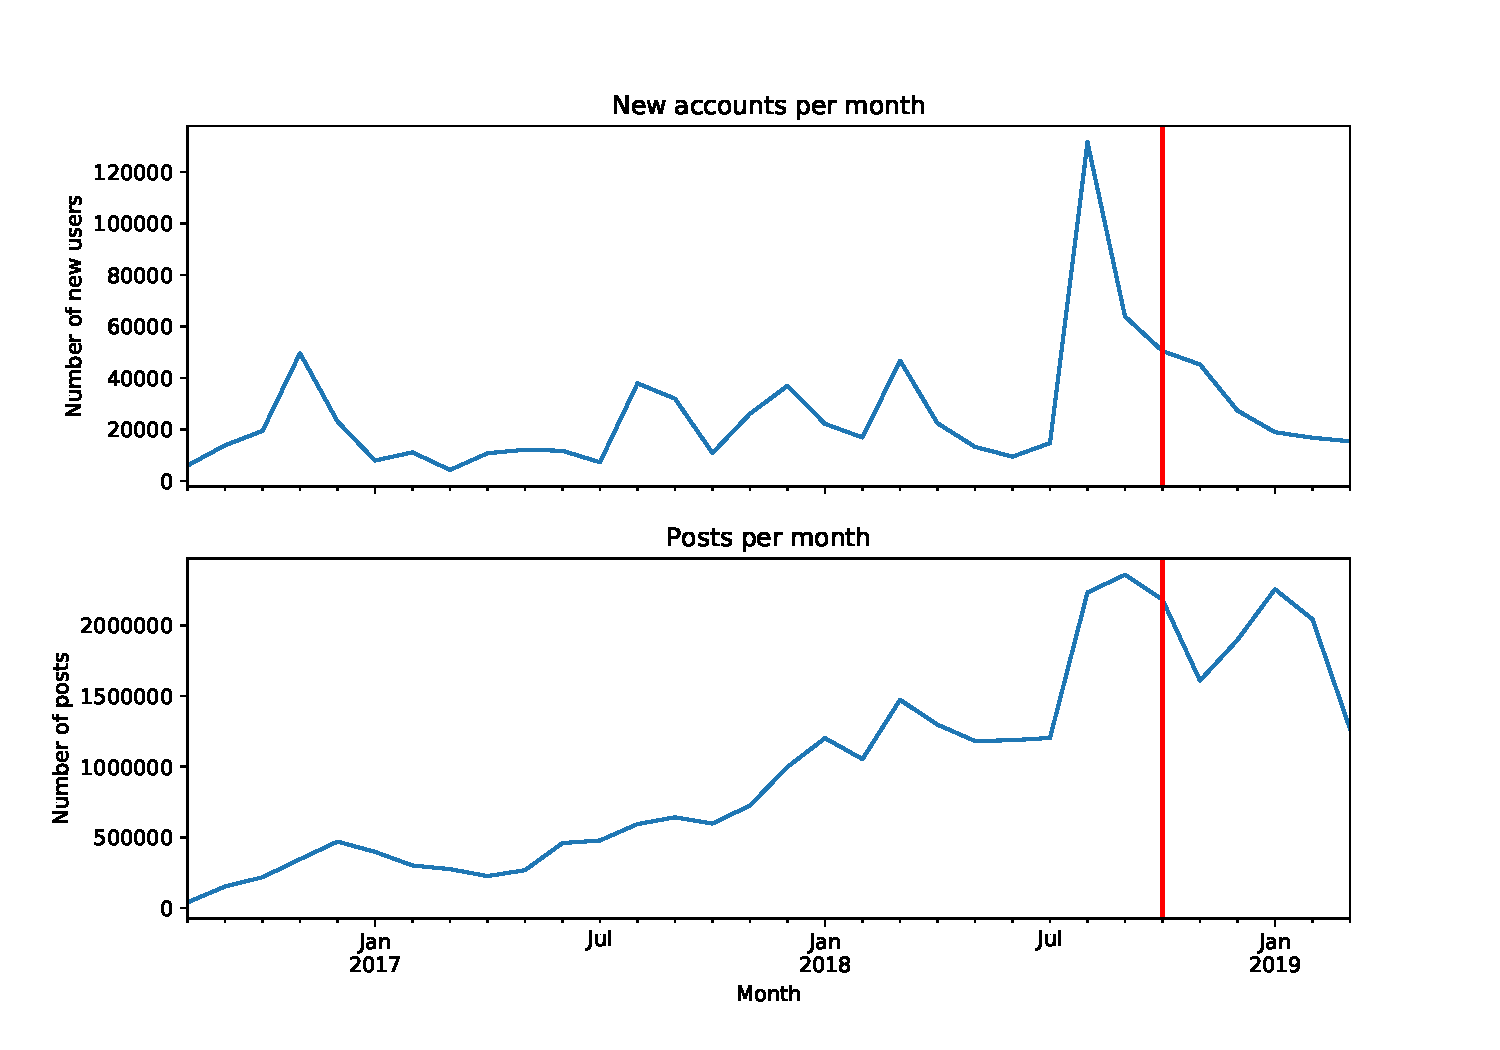
\includegraphics[width=\textwidth]{Before_and_after_counts.pdf}
	\caption{Site usage, with the shooting indicated with the red line}\label{over_time}
\end{figure}


\subsection{Data Pre-prepossessing}

The data collected on \textit{Gab} are very powerful in their completeness, but this makes converting them into a usable form difficult. Initially I tried using the standard \textit{NLTK} \cite{loper2002nltk} tokenizing tools. But I found these struggled with parsing the heavily non-standard spelling, and spacing conventions on \textit{Gab}, which with its longer than \textit{Twitter} character limit has many more posts with newlines, indented content and usage of emojis as separators or punctuation. Thus to parse and tokenize I ended up using a regex instead.

\subsection{Attempted methods}

I was hoping to use dynamic topic models in this work \cite{blei2006dynamic}, but was never able to get them to yield useful results. I attempted with the two implementations first the pure Python one by \textit{gensim} \cite{rehurek_lrec} which was far to slow on even $\frac{1}{32}$ of the data. Then the Java version created by Ble, et al \cite{blei2006dynamic}, which was able to analysis my test set in only three few days, but when run on the full dataset did not complete within eight days. I also did train a couple vanilla LDA models, but the resulting topics were not very good and they still took a couple days to complete. The large run times of the topic models I believe is due to the shape of the data, topic models are traditionally run on corpora with many words per document, and relatively few documents. While my data have many documents (posts) and few words per document. One avenue of further work is to see how if combining documents, such as by grouping all posts by author per month, would improve performance and interpretability. 

I was also hoping to use  the change point detention model \cite{kulkarni2015statistically}, but found it had already been done on \textit{Gab} to look at hate speech and anti-Semitism \cite{finkelstein2018quantitative}. This combined with me running low on time meant I did not do it.

\section{Results}

The code used for this project can be found ar \href{https://github.com/reidmcy/csc-2611-final-project}{github.com/reidmcy/csc-2611-final-project}, there is also a much larger private repo that was for previous work, along with some continuing projects and shows the commit history, access can be provide to this upon request. 

\subsection{Ngrams}

The first line of inquire was counting word occurrence an co-occurrence over time. This ngram analysis was done by binning the posts by month, then counting all unigrams, bigrams, trigrams and tetragrams. These were then filtered to remove, ones with hashtags and @ mentions. I also discard the tetragrams from my analysis as they proved to be very noisy and trigrams are the more common tool. Figure \ref{ngrams} shows the number of unique ngrams overtime of each type.


\begin{figure}[h!]
	\centering
	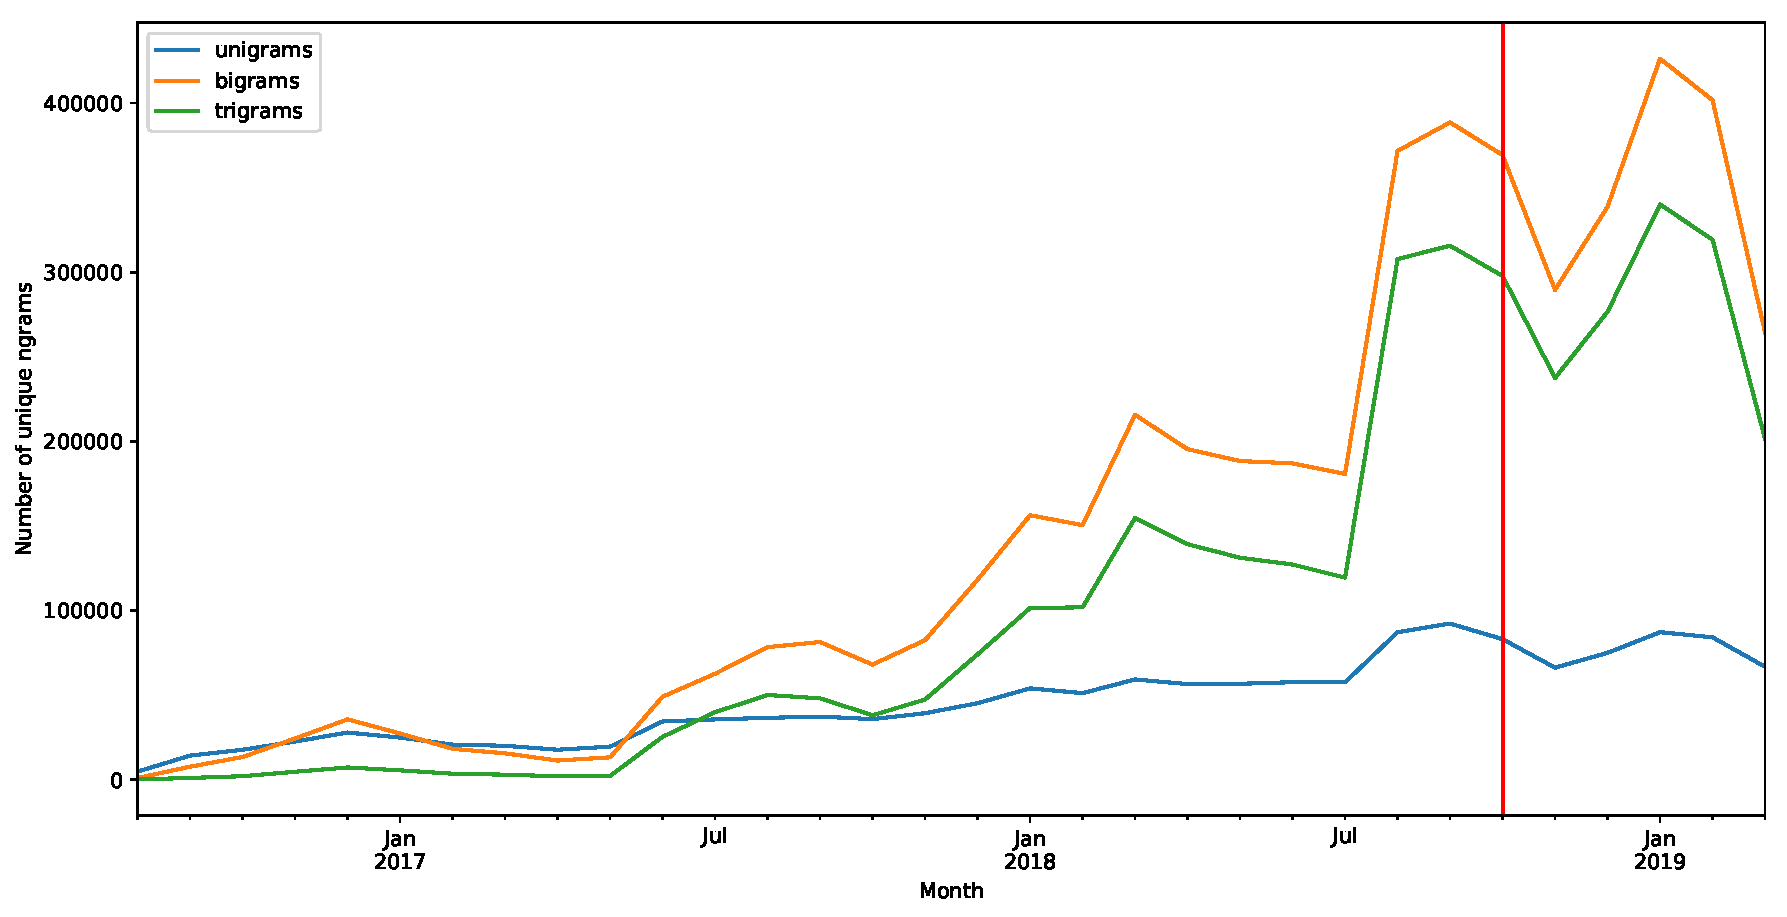
\includegraphics[width=\textwidth]{ngrams_overtime.pdf}
	\caption{Number of unique ngrams over time, shooting date marked with a line}\label{ngrams}
\end{figure}

The top new trigrams each month, with new meaning not being top in a previous month, are shown in figure \ref{top_tri}. The spiky nature of the occurrences shows that the discussion on the site would change quickly month to month. This makes the work usage generally more variable month to month. 

\begin{figure}[h!]
	\centering
	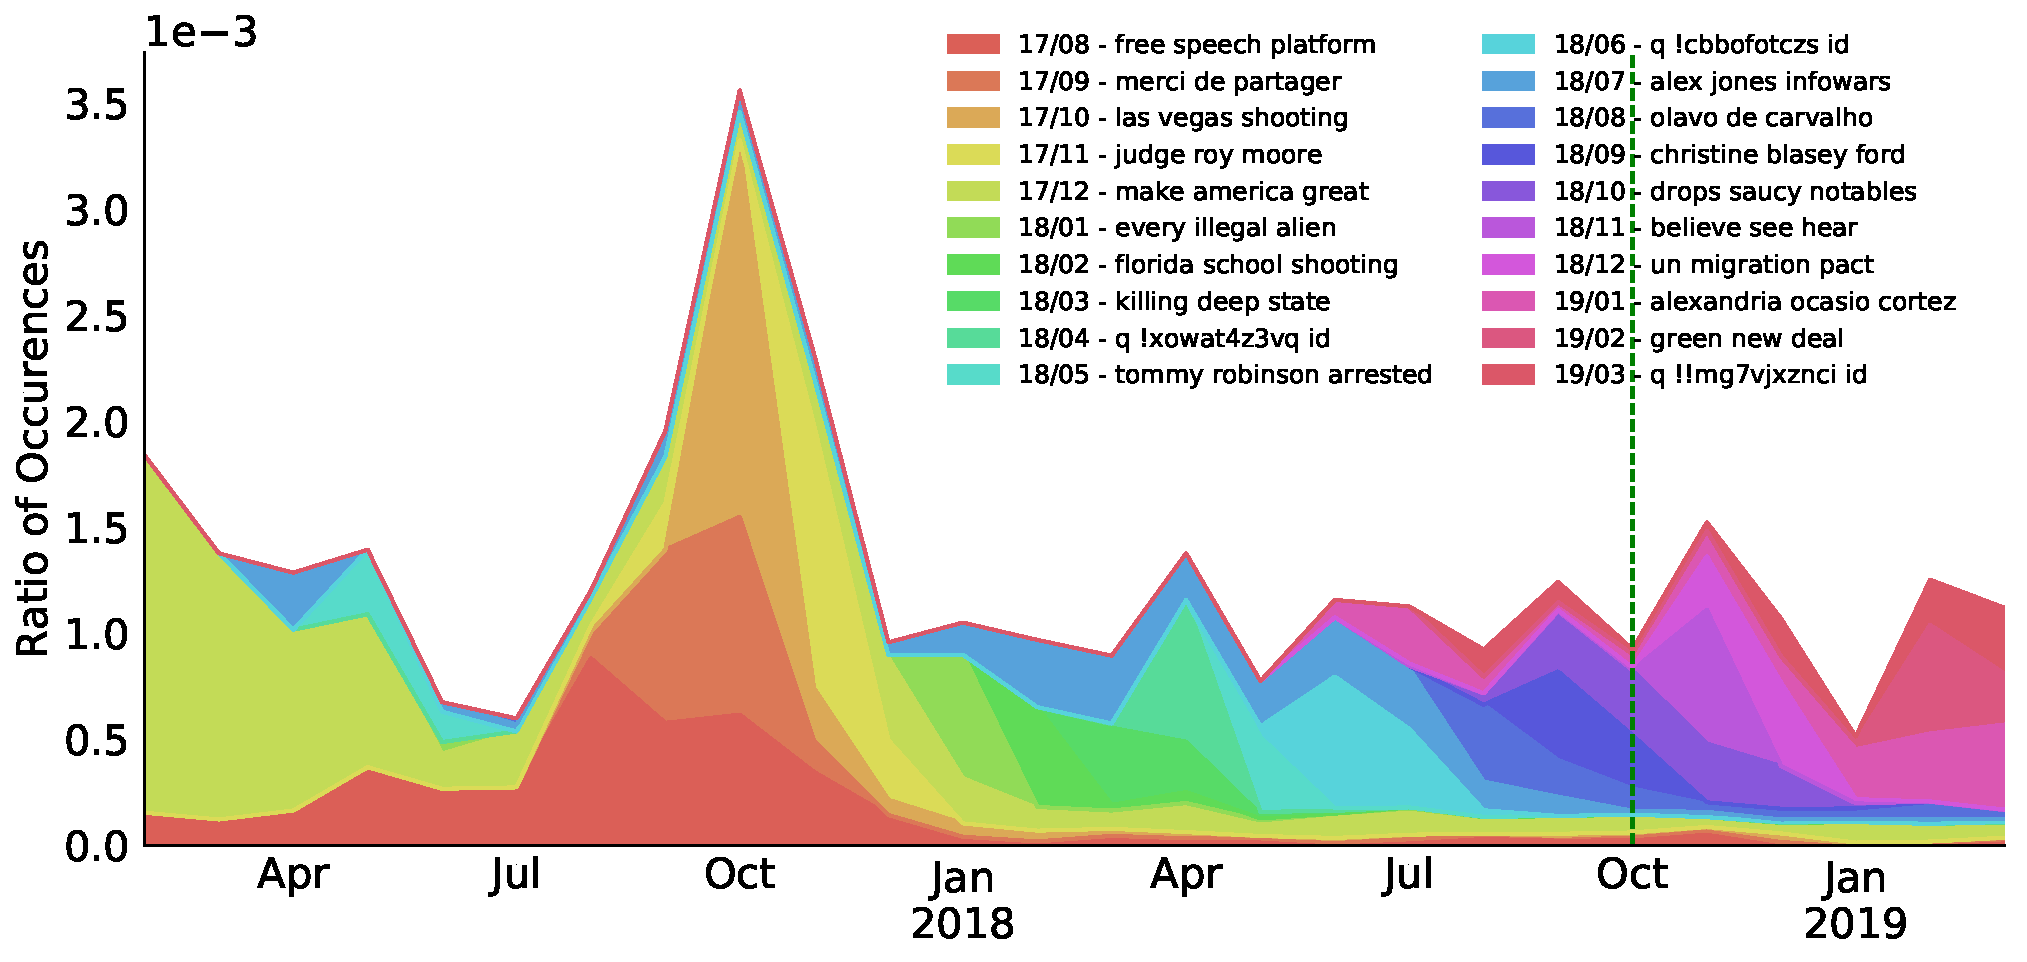
\includegraphics[width=\textwidth]{trigrams_norepost.pdf}
\caption{By month top new trigrams, with the shooting indicated with the line}\label{top_tri}
\end{figure}

To establish if the shooting had an effect on ant-Semtic langauge used on \textit{Gab}, I looked at the rate of usage of the top 5 (by count the anti-Semitic terms. The terms are from \textit{hatebase.org} \cite{hatebase}. Figure \ref{top_anti} shows that usage of some terms increased quickly after the shooting, but this did not last. Interestingly the word `jew' became much more frequent on \textit{Gab}, with table \ref{jew_table} showing the top trigrams containing `jew', the before corpus is more than twice as large so the null-hypostasis would be for the counts to be half as large as before, which is not the case at all.

\begin{figure}[h!]
	\centering
	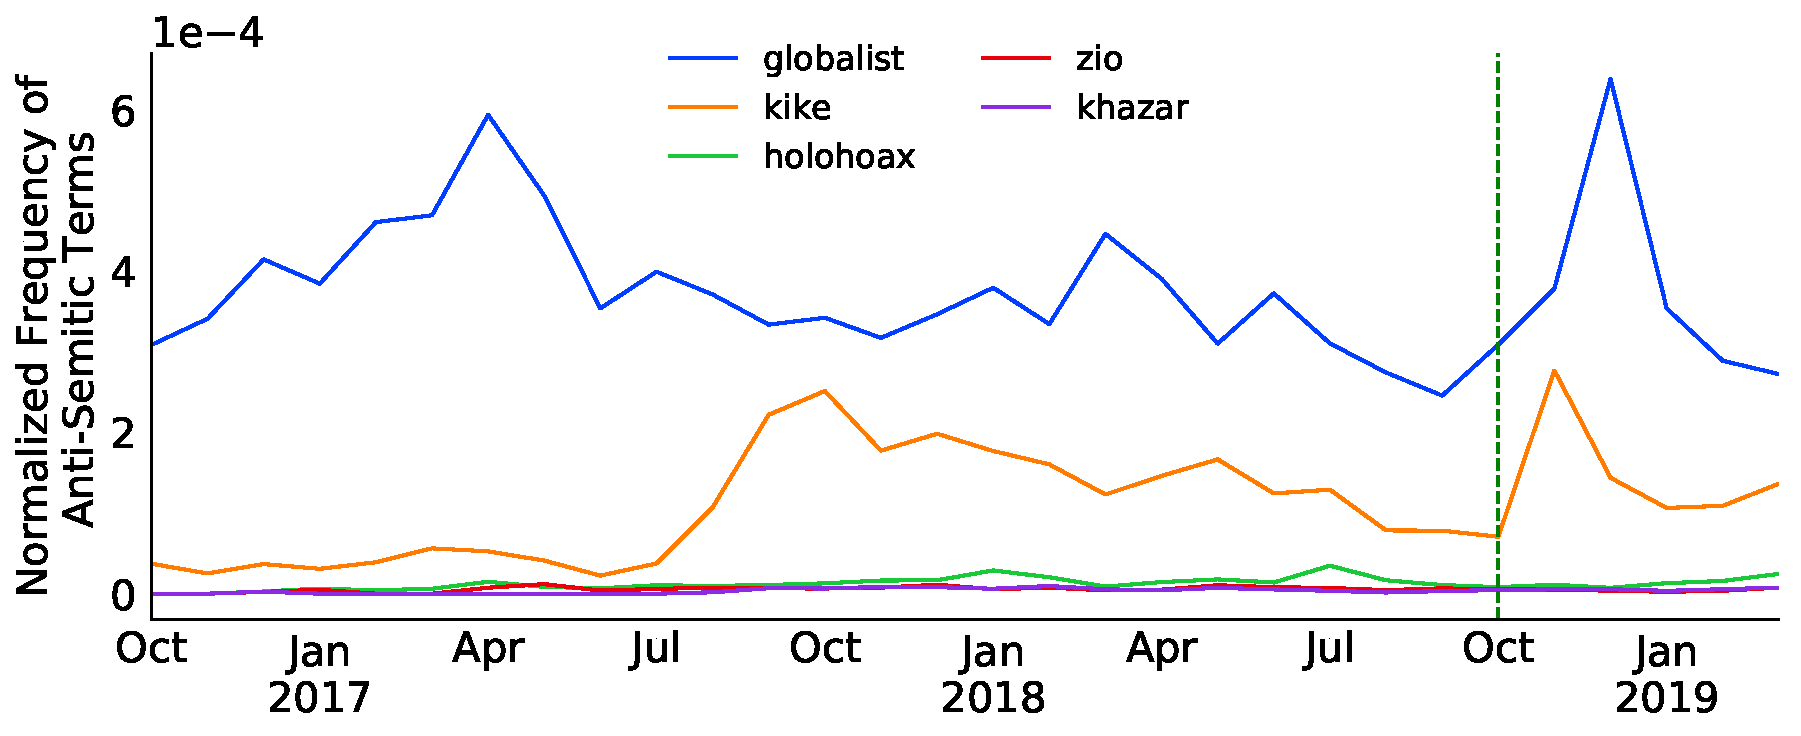
\includegraphics[width=1\textwidth]{overtime_normalized_antisem.pdf}
	\caption{By month ratio of occurrence of the top 5 anti-Semitic words via hatebase.org, with the shooting indicated with the  line}\label{top_anti}
\end{figure}

\begin{table}[h!]
	\centering
	\begin{tabular}{lrrr}
		\toprule
		Before words &count  & After words & count\\
		\midrule
		jew,world,order&582&jewish,conservative,journalist&2701\\
		anti,white,jewish&531&speaking,jew,hatred&1349\\
		white,jewish,activist&493&jew,hatred,sharia&1349\\
		already,taken,jewtube&331&simply,american,jewish&1348\\
		serious,question,jewish&322&american,jewish,conservative&1348\\
		question,jewish,groups&322&genetic,jewesses,jews&487\\
		six,million,jews&252&nit,jew,islamist&426\\
		000,000,jews&239&jew,haters,gab&402\\
		jews,support,country&236&majority,jews,support&395\\
		jew,jew,jew&234&vast,majority,jews&367\\
		genetic,jews,jewesses&214&jew,world,order&339\\
		false,system,jews&211&jews,rape,kids&273\\
		\bottomrule
	\end{tabular}
\caption{Before and after counts of top trigrams containing `jew'}\label{jew_table}
\end{table}

Addition to anti-Semitic language I examined if language associated with the shooting had been affected. For some words, such as those shown if figure \ref{shooting} there was a temporary increase in frequency. But when the whole of the corpus was considered there is not a clearer pattern. Table \ref{new_old} shows the words with the largest log odds change before and after, with some filtering for spam already applied. The new and old words do not show a clear pattern and mostly seem to be affected by other events. 


\begin{figure}[h!]
	\centering
	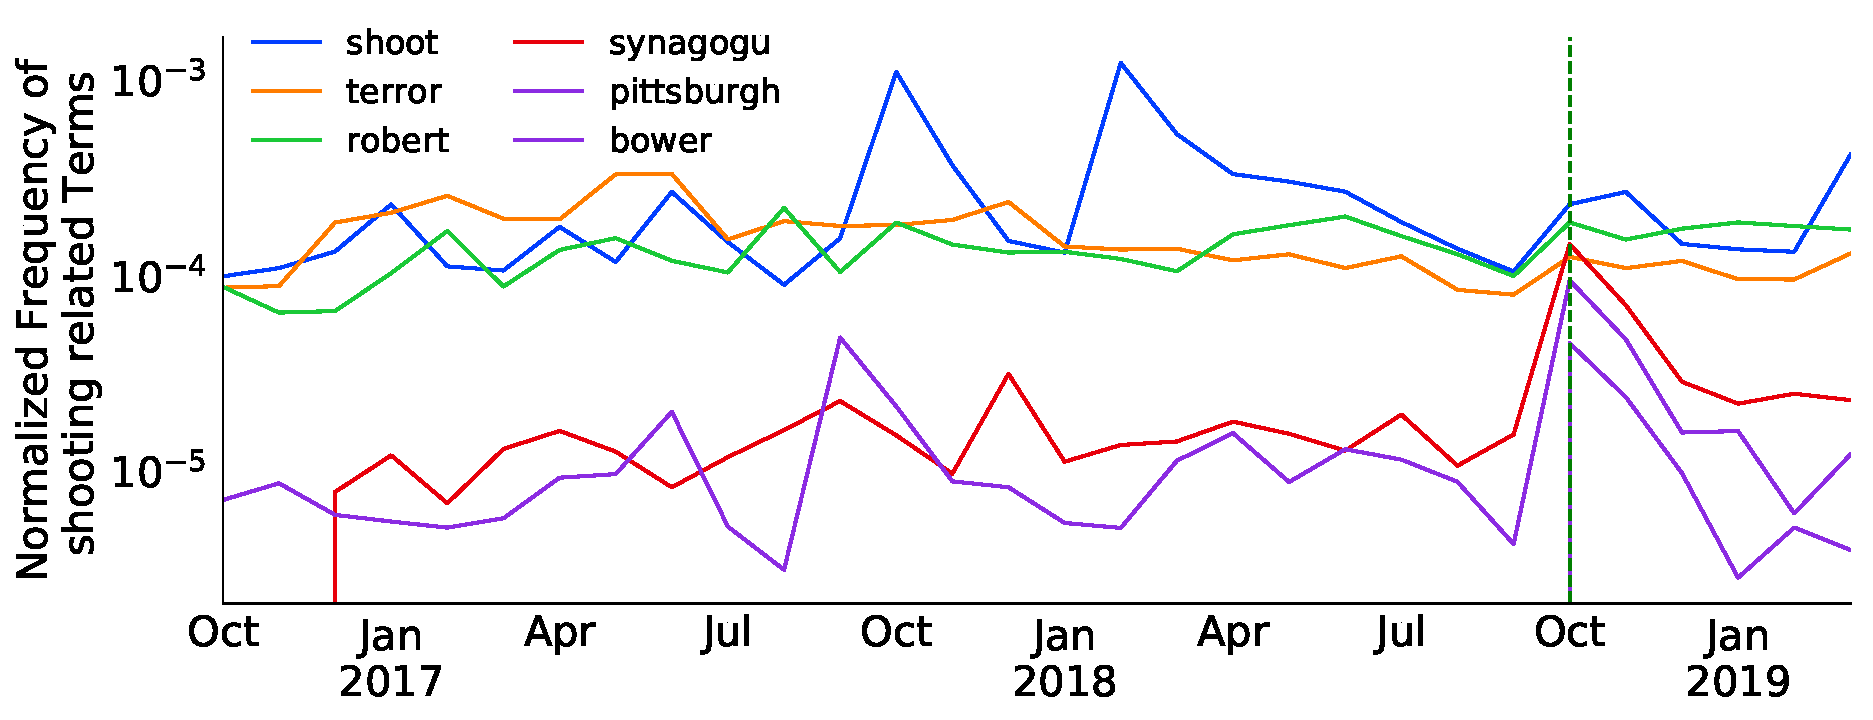
\includegraphics[width=1\textwidth]{overtime_shooting.pdf}
	\caption{By month ratio of occurrence of some shooting related words, with the shooting indicated with the  line. Note that the words were stemmed for the counting}\label{shooting}
\end{figure}

\begin{table}[h!]
	\centering
	\small
	\begin{tabular}{lr|lr}
		\toprule
		Word &  Log Odds &  Word  & Log Odds \\
		\midrule
		ballots         &   2.82517  &  gillette        &  -4.32011\\
		dec             &   2.68070  &  bonner          &  -4.12487\\
		broward         &   2.50657  &  christchurch    &  -3.93367\\
		oven            &   2.26191  &  alckmin         &  -3.83449\\
		nov             &   2.21719  &  ford’s          &  -3.64577\\
		compact         &   2.12065  &  candidatos      &  -3.49373\\
		thanksgiving    &   2.07243  &  covington       &  -3.48308\\
		acosta          &   2.01614  &  1d              &  -3.27645\\
		christmas       &   1.97001  &  candidato       &  -3.20228\\
		merry           &   1.85361  &  omarosa         &  -2.63009\\
		december        &   1.77640  &  uol             &  -2.60407\\
		macron          &   1.76386  &  marina          &  -2.59409\\
		\bottomrule
	\end{tabular}
	\caption{Words with the lowest and highest log odds of occurring in After from the top 10,000 words by count in After}\label{new_old}
\end{table}

\subsection{Word2Vec}

To see if shifts in meaning could be detected I created a series of word2vec \cite{mikolov2013efficient} models using \textit{gensim}\cite{rehurek_lrec}. These were trained on the posts before the shutdown, those after the shutdown and on each month separately. To tun the models I conducted the standard analogies tasks on, finding a window size of 10, using hierarchical softmax and 512 dimensions performed best after a basic grid search. For this analysis though I used 300 dimensions as performance difference is small and it allows me to use the Google News word2vec pre-trained embeddings. I also trained a word2vec model on all \textit{reddit} posts from October 2018 to use as a baseline in comparisons.

My first attempt at seeing the semantic change of words was to use the procrustes aliment procedure \cite{hamilton2016diachronic}. Where each embedding is aligned to the previous one. When done monthly the results proved to be very noisy on the words I considered, such as `jew' or `liberal'. I believe this is mostly due to the size of the training data. Some months would have a cosine difference of 0, and the next month would be 1, with no pattern and when the order of alignments was changed (I tried aligning sequentiality starting at each month, and wrapping around to the first when necessary) the difference would be completely different.

To combat the noise I used the Google News word2vec pre-trained embeddings as a stable basis and aligned all my models to it, so it was unchanged after each alignment. This proved to lead to much less noise, although it means the measurements are now blind to shifts within a hypersphere defined by equal cosine difference from a point in Google News word2vec pre-trained embeddings space.

The results of the newly aligned word2vecs were also quite noisy, figrue \ref{randaling} shows the cosine distance of words from their values in the Google News word2vec. You can see that month  to month they shift by up to .2 with very little pattern and that all are very far away from the Google News word2vec originals. I also looked at some specifically sensitive terms to see if they also had the same pattern, figure \ref{eth}. It is interesting that the terms such as `women' or `black' are more similar than `computer' to the Google News word2vec originals, suggesting that they are weighted higher in the alignment and that less sensitive words may be more divergent.

\begin{figure}[h!]
	\centering
	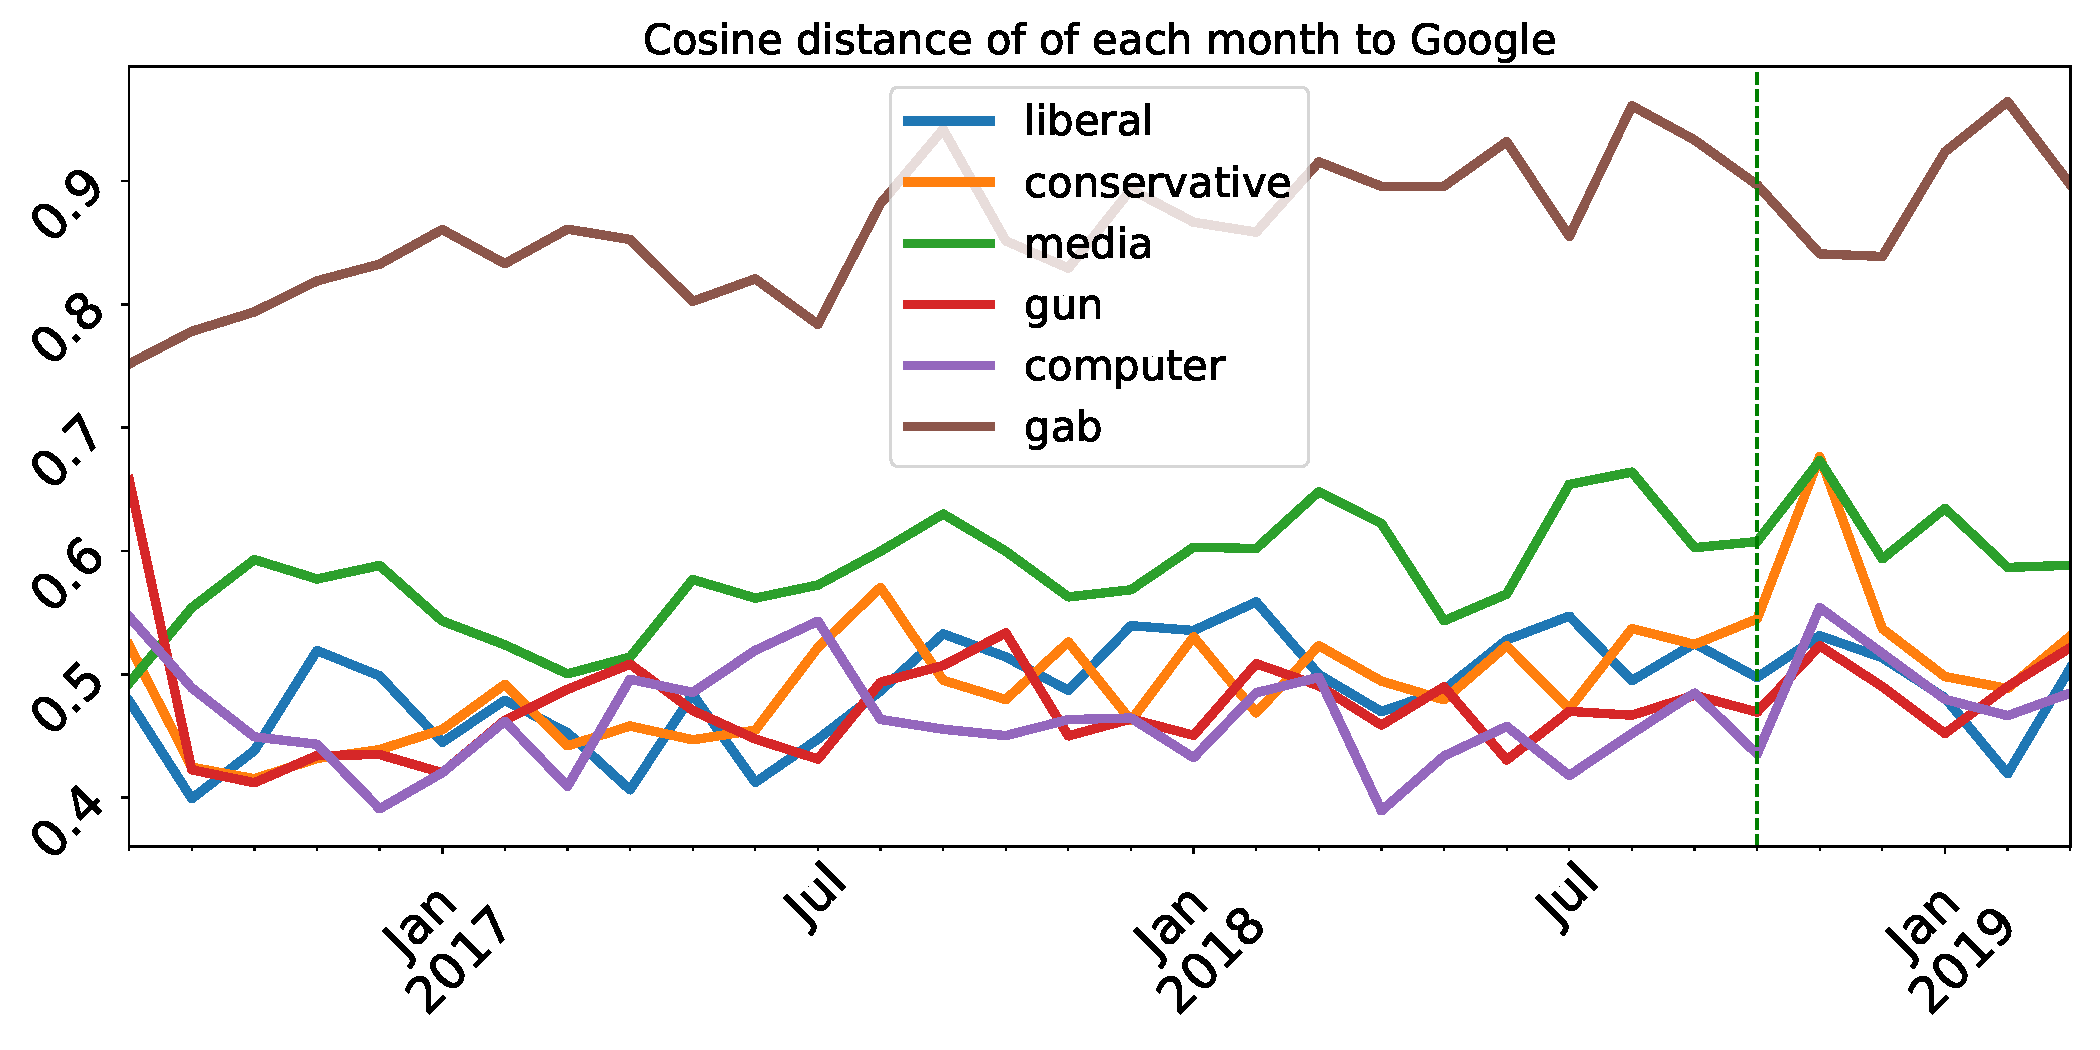
\includegraphics[width=1\textwidth]{sim_misc_jewish.pdf}
	\caption{By month cosine distance of select words from their values in the Google News word2vec }\label{randaling}
\end{figure}

\begin{figure}[h!]
	\centering
	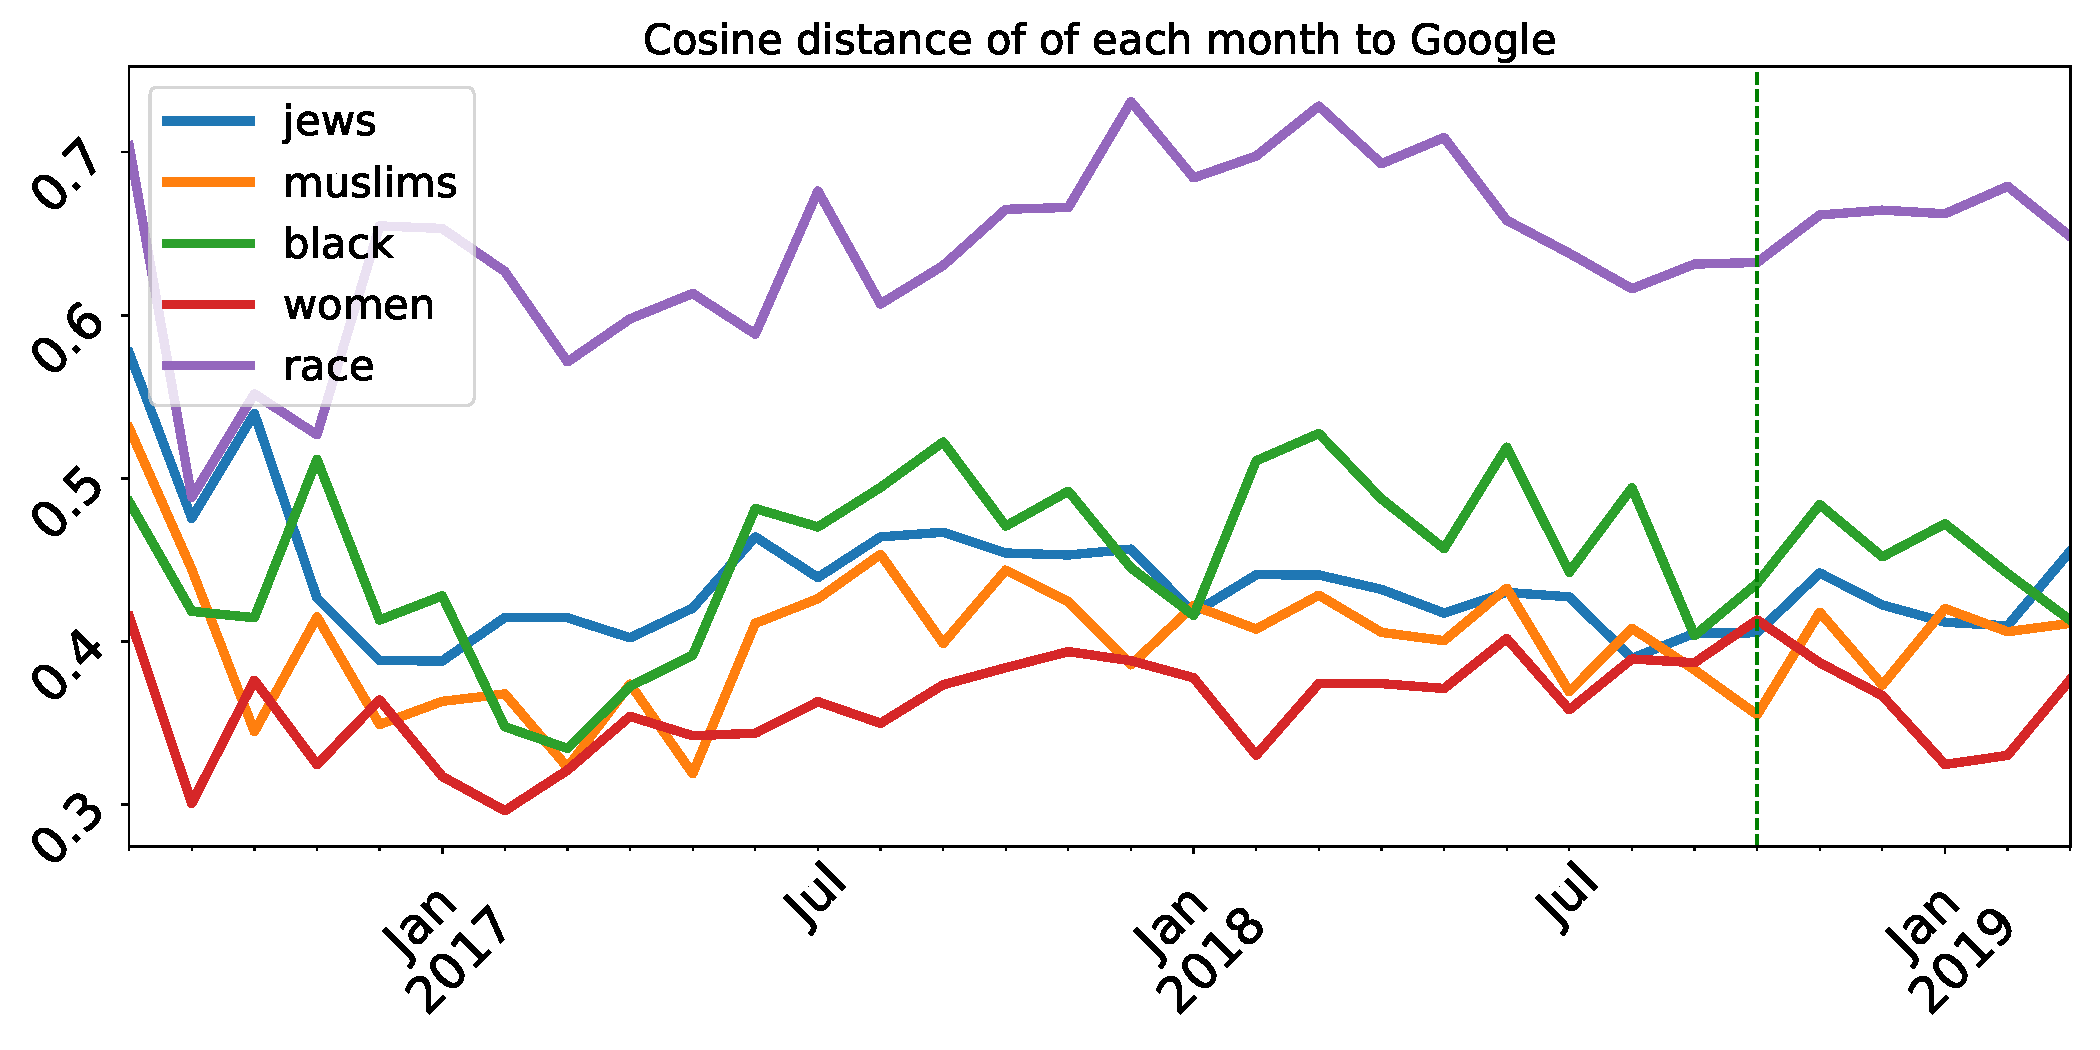
\includegraphics[width=1\textwidth]{sim_ethnic_jewish.pdf}
	\caption{By month cosine distance of select ethnic words from their values in the Google News word2vec }\label{eth}
\end{figure}

To looking at specifically words related to anti-Semitism I found the nearest 3000 neighbours in Google News and looked at the top words also share by the Before. After and \textit{Reddit} word2vecs. Figure \ref{dist2} shows their cosine distances to the Google News. An alternative way to view this is by doing a t-SNE (on the top 10,000 words) and reducing to two dimensions the space, this is then a two dimensional measure that will not have the issue of not being sensitive to rotations in a hypersphere that the previous measures do, but it does have the much large downside of using information destroying dimension reduction, figure \ref{tsne} shows how the words shift. That the blue and green lines have nearly perfect overlap shows that the before and after semantics of those words did not shift much. 

\begin{figure}[h!]
	\centering
	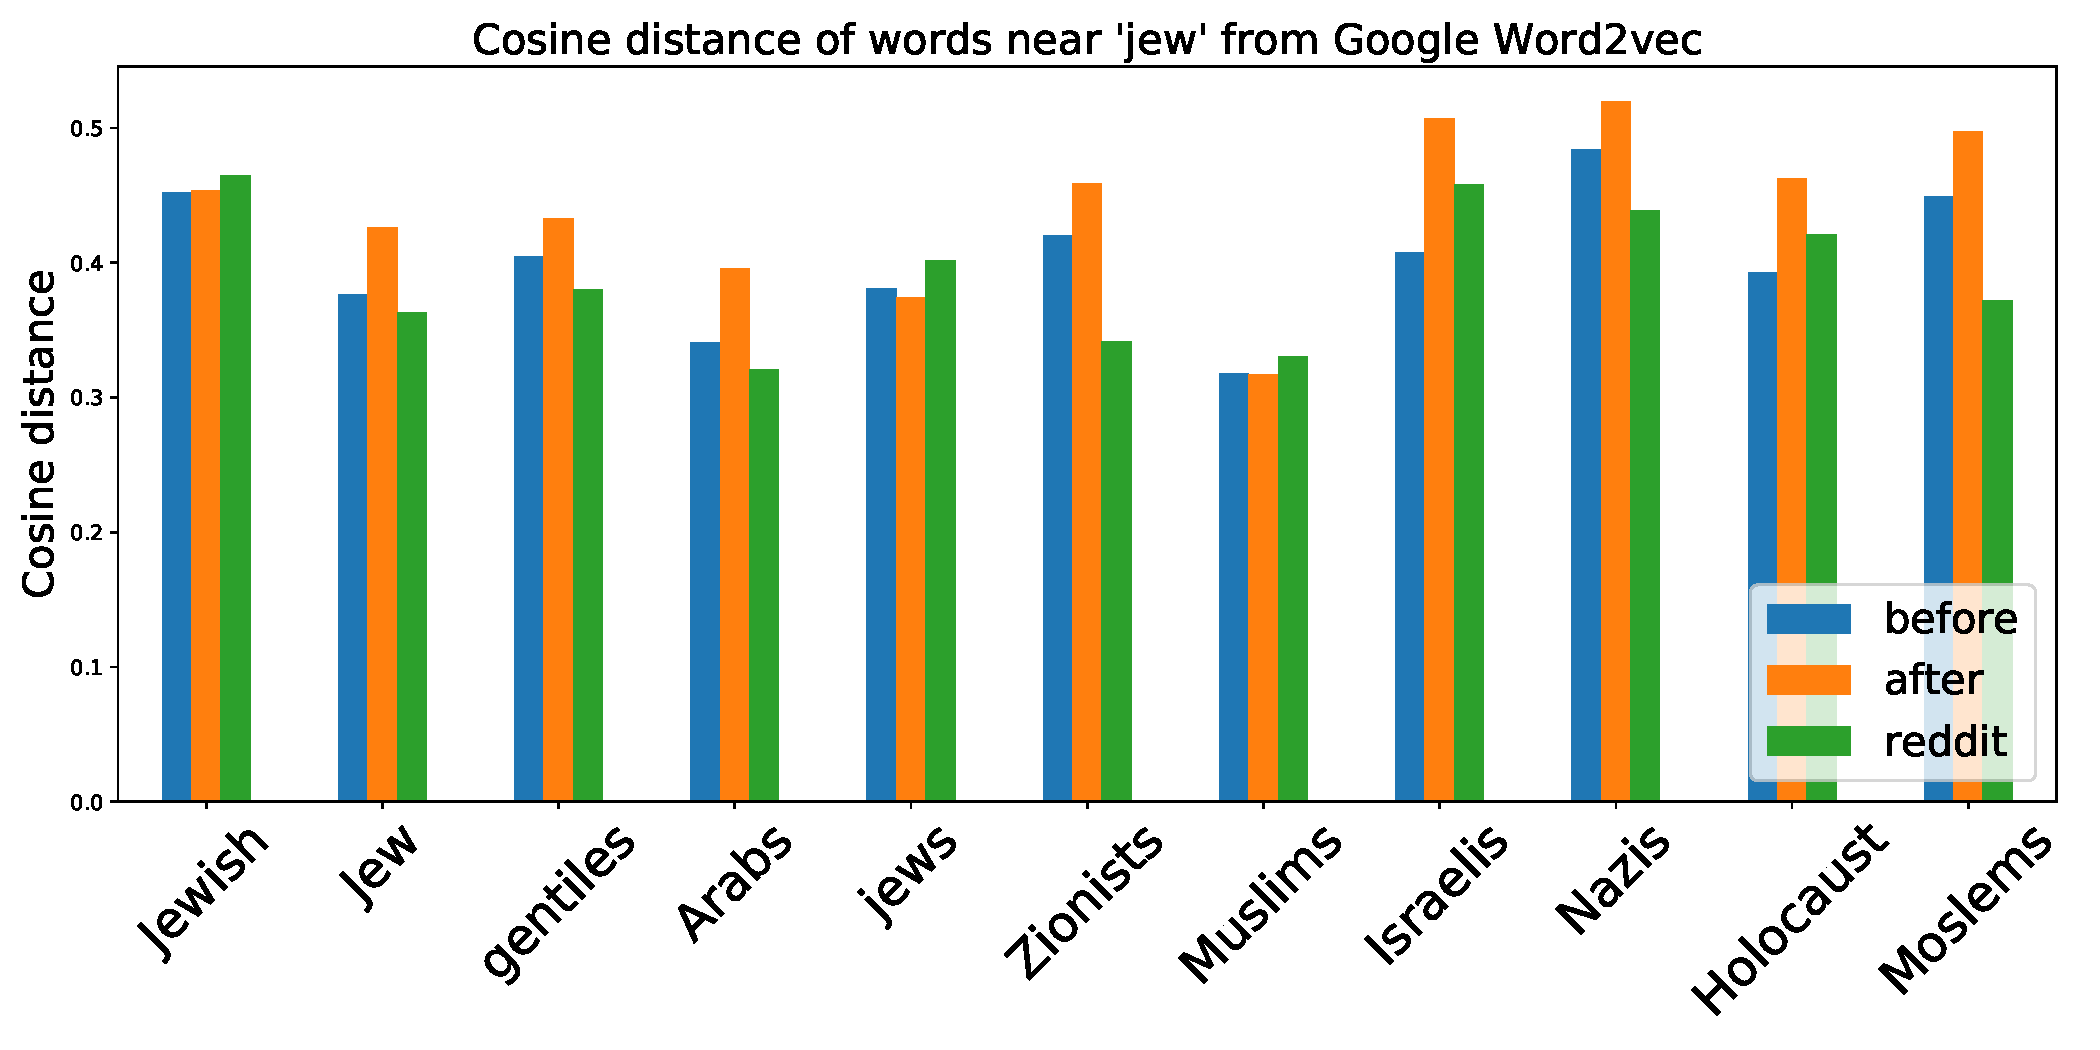
\includegraphics[width=1\textwidth]{sim_bars_jewish.pdf}
	\caption{Cosine distance of different words from Google to aligned word2vecs}\label{dist2}
\end{figure}

\begin{figure}[h!]
	\centering
	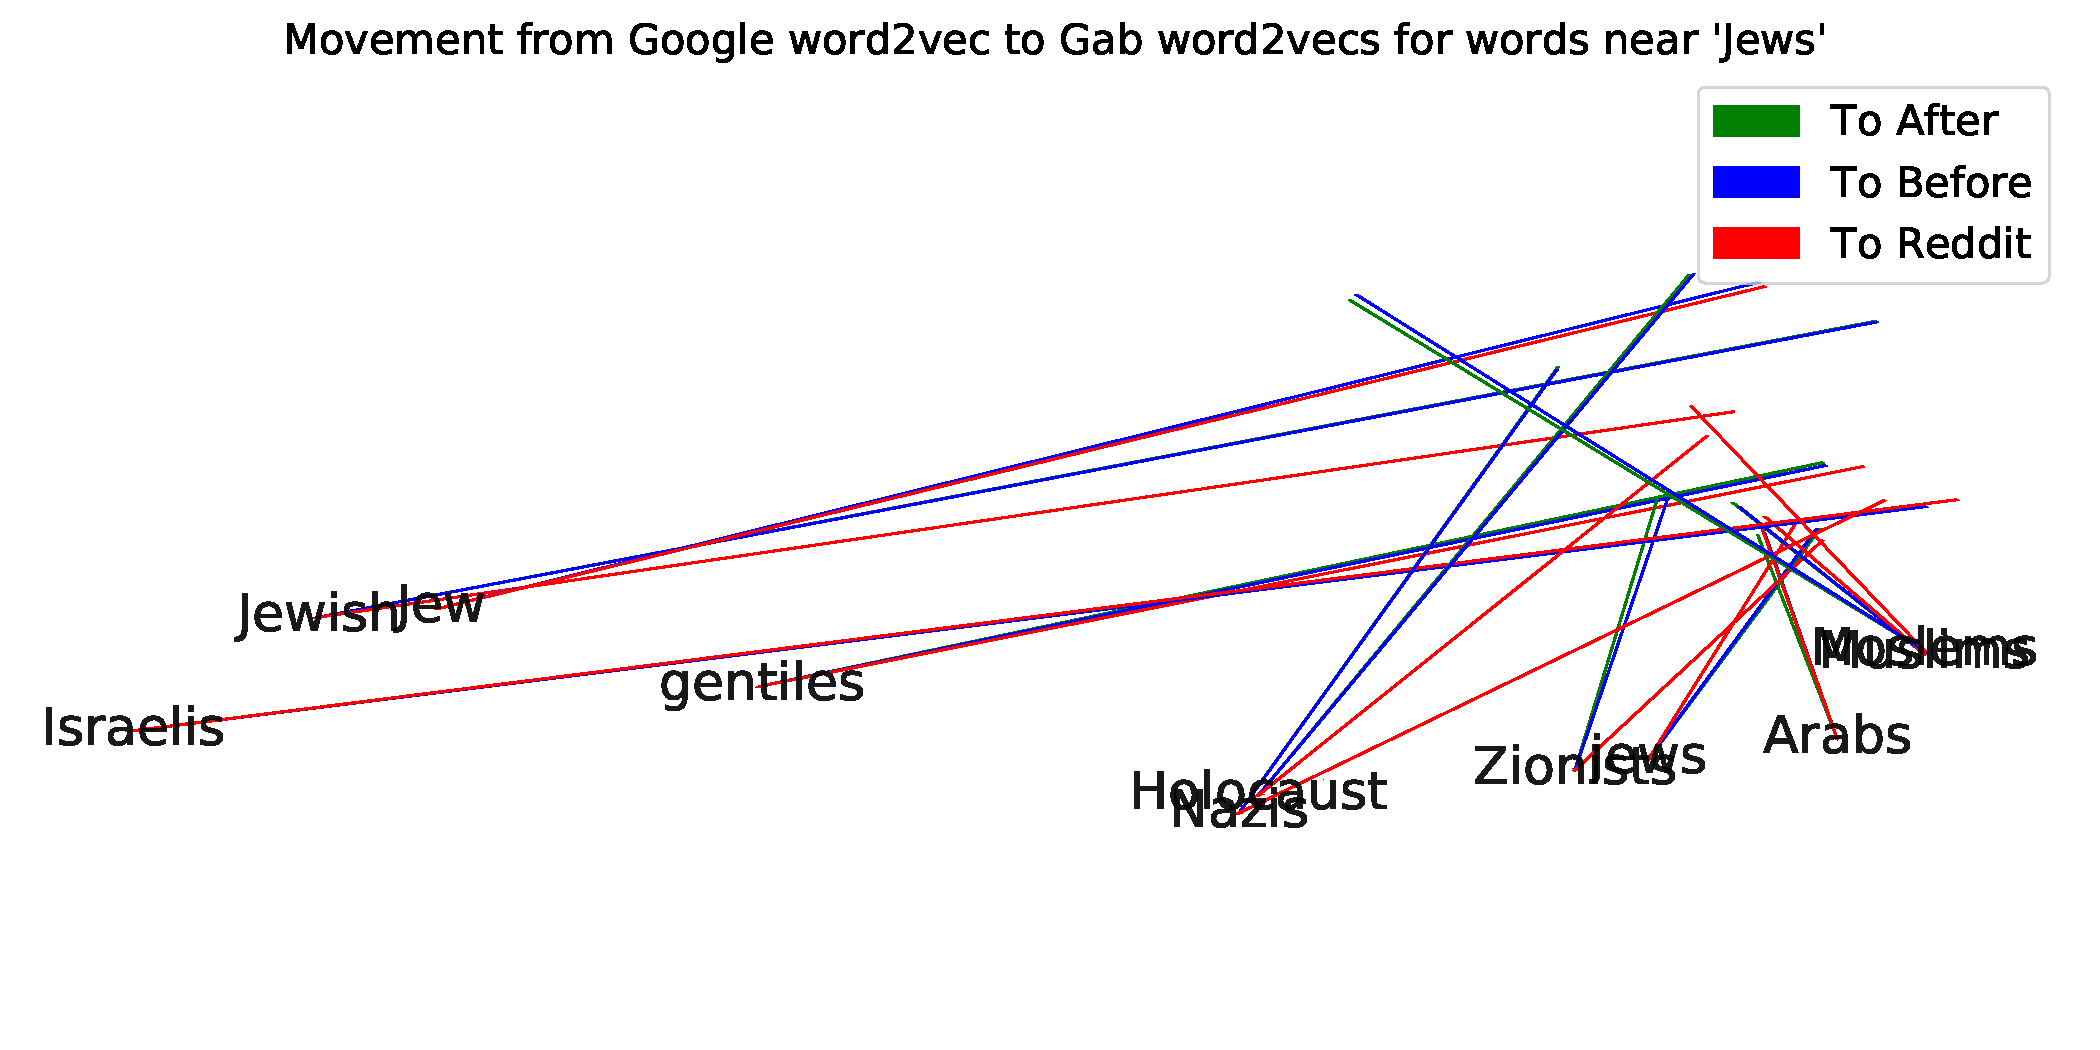
\includegraphics[width=1\textwidth]{tsen_jewish_arrows.pdf}
	\caption{t-SNE embedding of all 4 aligned word2vecs, lines show movement from Google to to other Word2Vecs}\label{tsne}
\end{figure}


\section{Discussion}

In this report I showed that there was a measurable shift in the language usage on \textit{Gab} immediately after the shooting, but that it was likely temporary. The shift was also mostly in word frequencies and I was not able to provably identify any real semantic change. This lack of provability is due to two main factors, one the lack of a control and two the small size of the data. Future work could be done with holdout sets and randomization to start getting error bars along with simply having more data. The word usage change I was able to find maths other work \cite{finkelstein2018quantitative} on the matter and suggests that long term affects on the communities language will be minor. Thus more nuanced measure will have to be used to detect real semantic change.

The shifts in usage patterns to \textit{Gab} also suggest a substantial change in the community, the more ancillary members are leaving and only the true believers remain. The community also is more aware of it's observation by outsiders, and one thing I would like to see in the future is an analysis \textit{Gab}'s non-standard English. Some popular topics, such as conspiracy theories like Qanon \cite{qan}, lead to the creation of their own languages. These new words have bee used for a long time by political groups to communicate \cite{lopez2015dog} and under harsher scrutiny they may be getting more intense.

\bibliography{paper.bib}
\bibliographystyle{plain}
\end{document}
